\documentclass[12pt,a4paper,]{article}
\usepackage{lmodern}
\usepackage{amssymb,amsmath}
\usepackage{ifxetex,ifluatex}
\usepackage{fixltx2e} % provides \textsubscript
\ifnum 0\ifxetex 1\fi\ifluatex 1\fi=0 % if pdftex
  \usepackage[T1]{fontenc}
  \usepackage[utf8]{inputenc}
\else % if luatex or xelatex
  \ifxetex
    \usepackage{mathspec}
  \else
    \usepackage{fontspec}
  \fi
  \defaultfontfeatures{Ligatures=TeX,Scale=MatchLowercase}
\fi
% use upquote if available, for straight quotes in verbatim environments
\IfFileExists{upquote.sty}{\usepackage{upquote}}{}
% use microtype if available
\IfFileExists{microtype.sty}{%
\usepackage{microtype}
\UseMicrotypeSet[protrusion]{basicmath} % disable protrusion for tt fonts
}{}
\usepackage{hyperref}
\hypersetup{unicode=true,
            pdfborder={0 0 0},
            breaklinks=true}
\urlstyle{same}  % don't use monospace font for urls
\usepackage{graphicx,grffile}
\makeatletter
\def\maxwidth{\ifdim\Gin@nat@width>\linewidth\linewidth\else\Gin@nat@width\fi}
\def\maxheight{\ifdim\Gin@nat@height>\textheight\textheight\else\Gin@nat@height\fi}
\makeatother
% Scale images if necessary, so that they will not overflow the page
% margins by default, and it is still possible to overwrite the defaults
% using explicit options in \includegraphics[width, height, ...]{}
\setkeys{Gin}{width=\maxwidth,height=\maxheight,keepaspectratio}
% Make links footnotes instead of hotlinks:
\renewcommand{\href}[2]{#2\footnote{See \texttt{\url{#1}}}}
\setlength{\emergencystretch}{3em}  % prevent overfull lines
\providecommand{\tightlist}{%
  \setlength{\itemsep}{0pt}\setlength{\parskip}{0pt}}
\setcounter{secnumdepth}{5}
% Redefines (sub)paragraphs to behave more like sections
\ifx\paragraph\undefined\else
\let\oldparagraph\paragraph
\renewcommand{\paragraph}[1]{\oldparagraph{#1}\mbox{}}
\fi
\ifx\subparagraph\undefined\else
\let\oldsubparagraph\subparagraph
\renewcommand{\subparagraph}[1]{\oldsubparagraph{#1}\mbox{}}
\fi

\date{}


%
% Line Spread, Page Markings & Hyperlinked Documents
%
\linespread{1.3}
% Margin:
\usepackage[top=1.5in, bottom=1.5in, right=1in, left=1in]{geometry}

% To silence too small headheight warning
\setlength{\headheight}{15pt}

% Header & Footer:
\usepackage{fancyhdr}
\pagestyle{fancy}
\fancyhf{} % Clear all header and footer fields
\fancyhead[LO,RE]{Helpdesk Ticketing System\\{\vspace{-2pt}\scriptsize Semester 1}}
\fancyhead[LE,RO]{\leftmark\\{\vspace{-4pt}\scriptsize SWE40001 Software Engineering Project}}
\fancyfoot[LE,RO]{\thepage\ifodd\value{page}\else\hfill\fi}
\usepackage{float}

\begin{document}

{
\setcounter{tocdepth}{3}
\tableofcontents
}
\newpage
\section{Goals \& Objectives}\label{goals-objectives}

Whilst reading this documentation, it is important to keep the following
goals and objectives in mind:

\emph{The Doubtfire Helpdesk Ticketing System will provide:}

\begin{itemize}
\tightlist
\item
  A way to improve efficiency of helping students
\item
  A way for tutors to track which students need help
\item
  A way to manage tutor clock-on times
\item
  A way for convenors to see how much their students utilise the
  helpdesk and at what times
\item
  A way for convenors to to see how their tutors are clocking on at the
  helpdesk
\end{itemize}

Refer to the extended planning documentation for more on this.

\section{Entities}\label{entities}


\begin{figure}[h!]
  \centering
  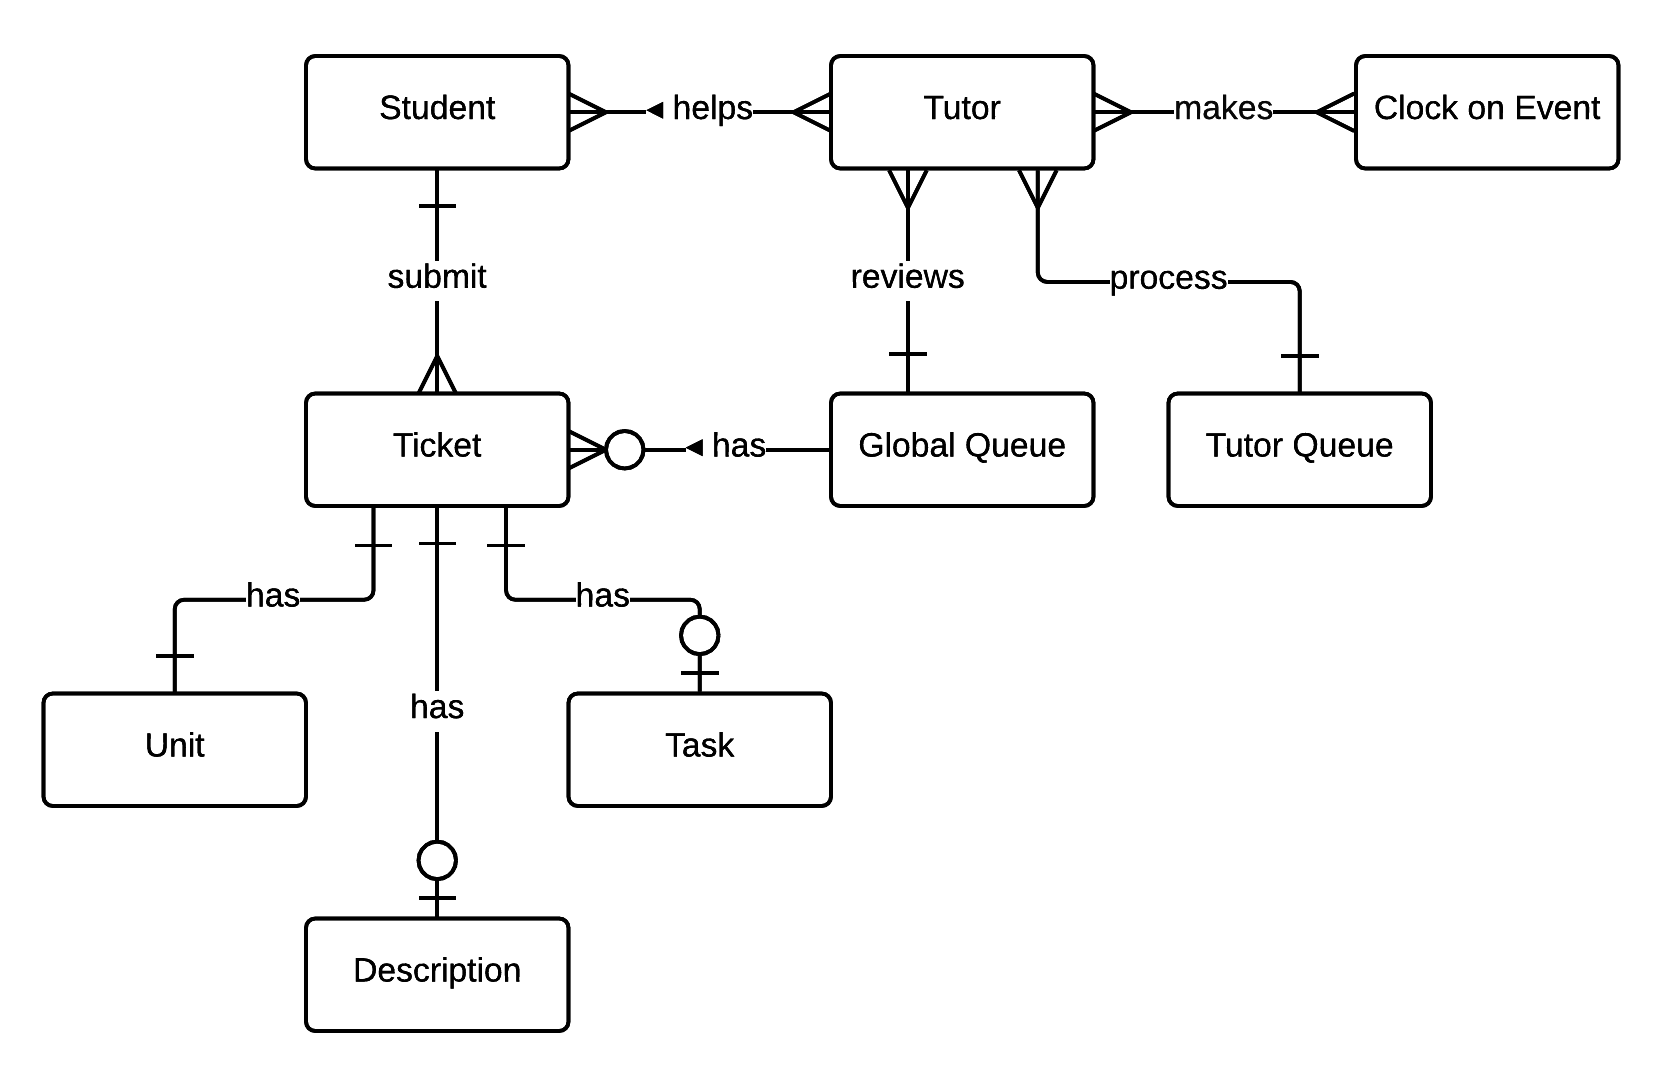
\includegraphics{5d0054b7-3365-4f00-a4a1-d29212ec68f0.png}
  \caption{Entity Relationship Diagram highlighting fundamental entities}
  \label{ed}
\end{figure}

Figure~\ref{ed} shows a basic ERD, highlighting the fundamental entities that the
helpdesk ticketing system works with.

There is a distinction between a \textbf{tutor's queue} and the \textbf{global queue}.

A \textbf{tutor's queue} is a group of a number of students that a tutor
rotates through as he/she helps those students at the helpdesk. It is
sorted by the \textbf{inverse} time the ticket was last reviewed by the
tutor (i.e., last reviewed a while ago or never reviewed at all first,
just reviewed a few seconds ago at the end etc.)

A \textbf{global queue} is a list of \emph{all unallocated tickets} that
have been submitted at the helpdesk. Tutors working at the helpdesk aim
to keep this global queue as minimal as possible; when a new ticket
comes to the global queue, tutor's may:

\begin{enumerate}
\def\labelenumi{\arabic{enumi}.}
\tightlist
\item
  accept a new ticket, which will move that ticket to the tutor's own
  queue or,
\item
  refer that ticket to another tutor, which will move that ticket to the
  referral's queue.
\end{enumerate}

\section{Use Cases}\label{use-cases}

Refer to a summary of use cases in Figure~\ref{uc}.

\begin{figure}
  \centering
  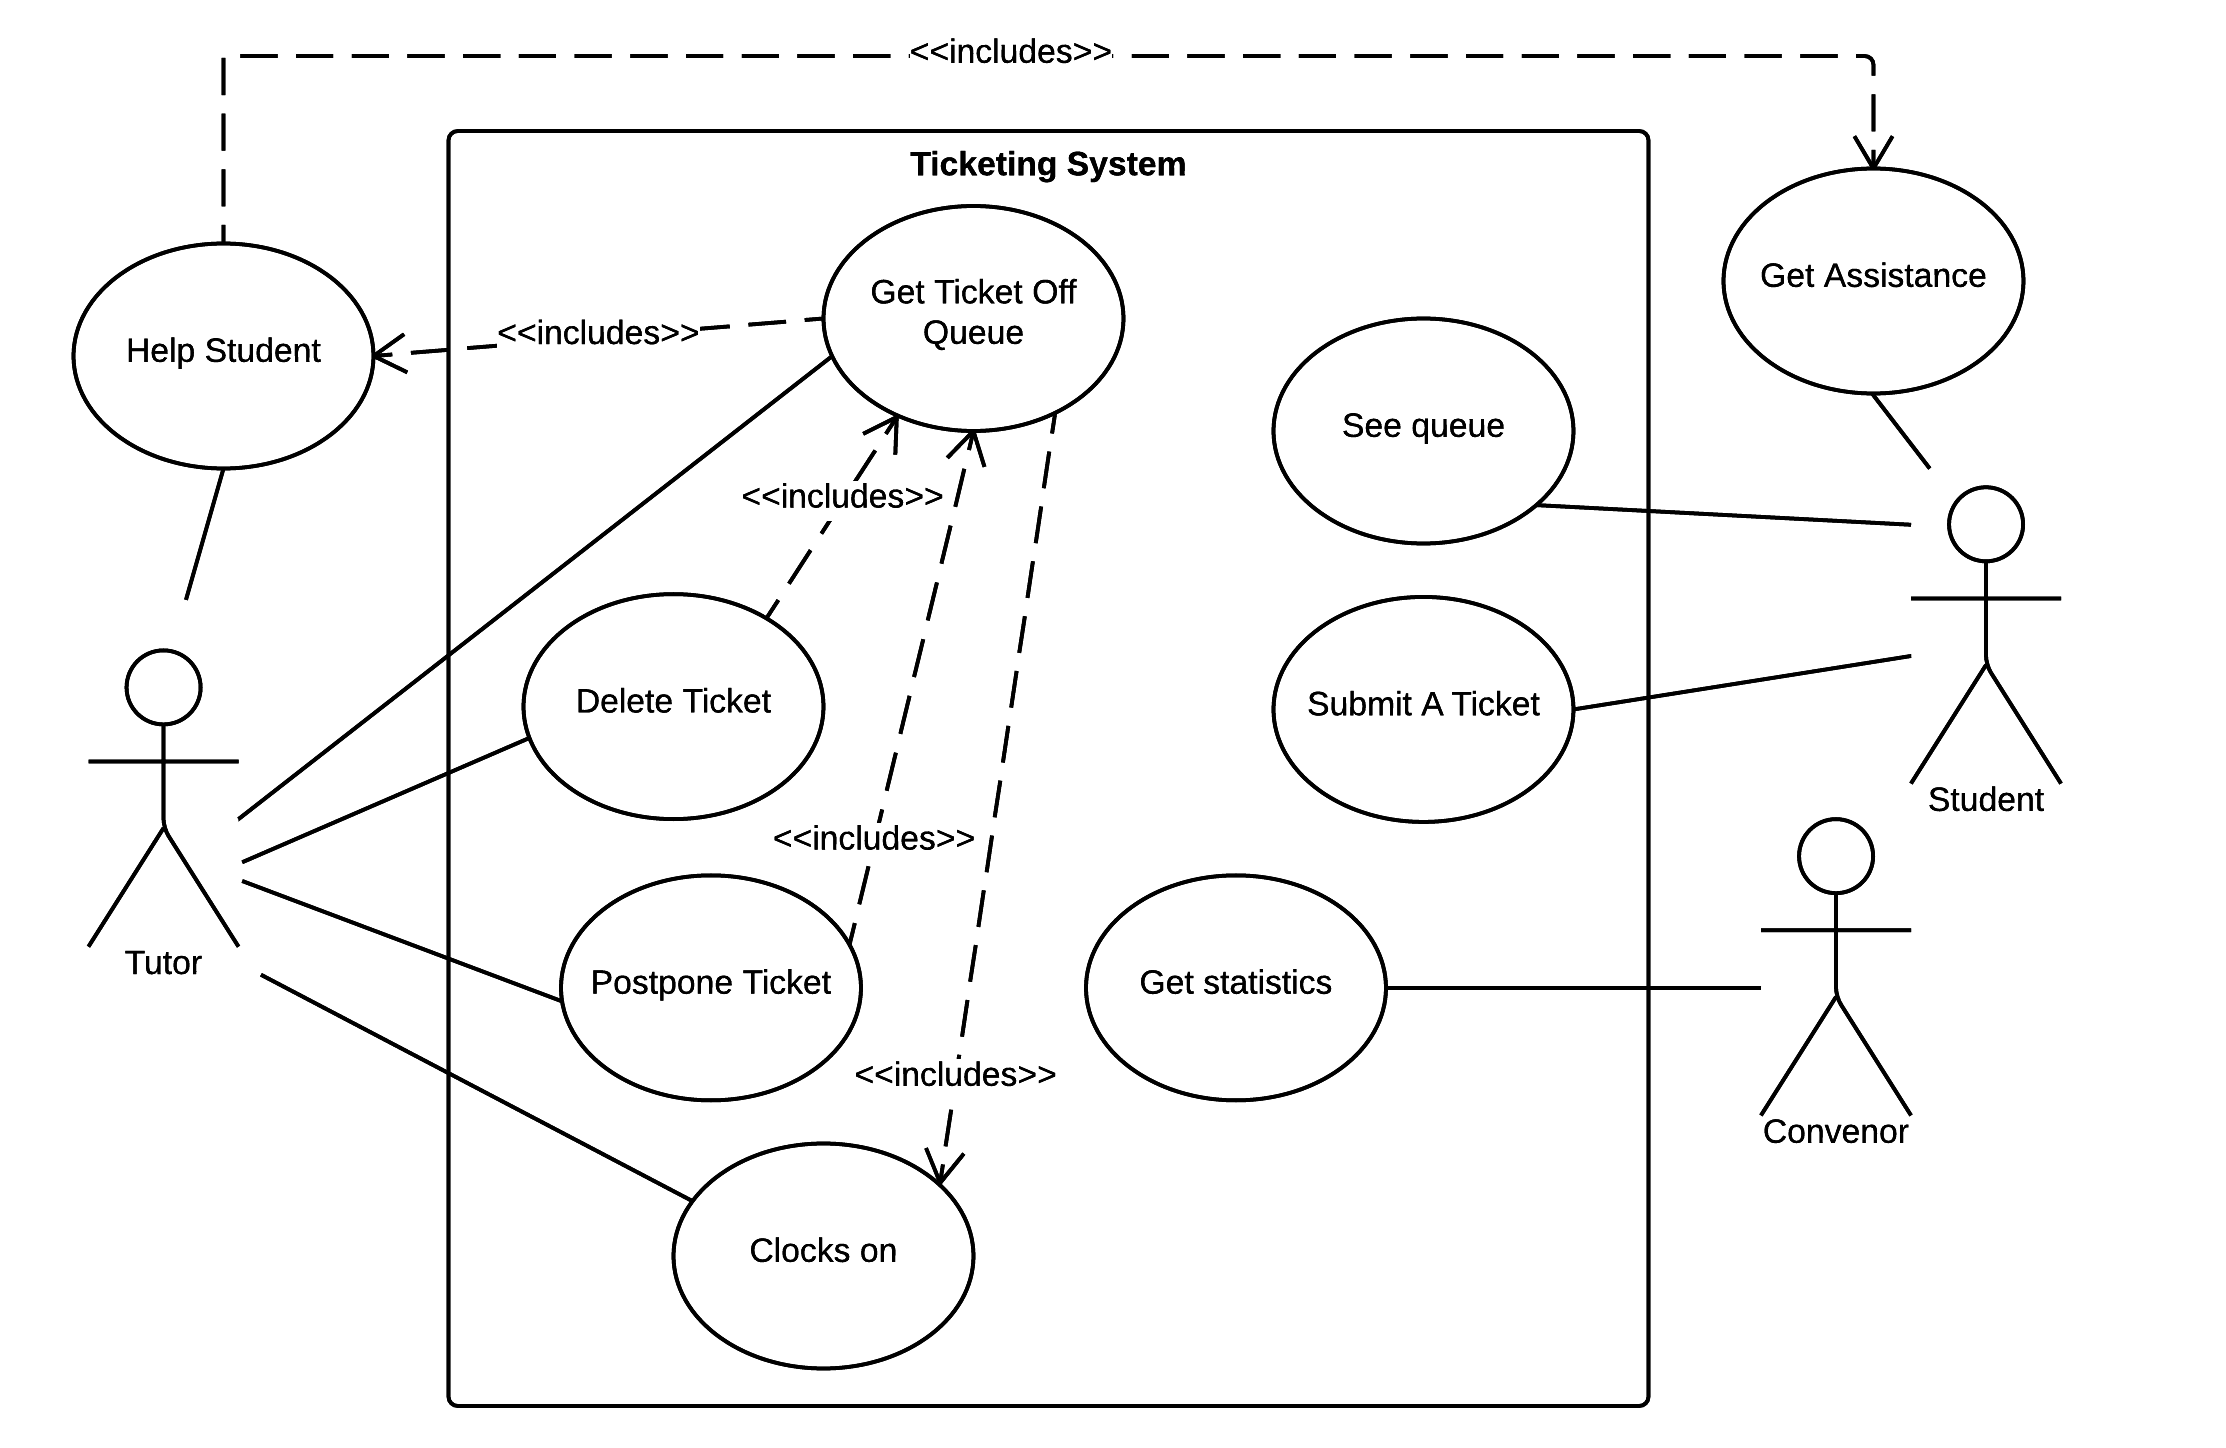
\includegraphics{8a6ccacc-322d-4611-af96-34ddbb8b820e.png}
  \caption{Summary of use cases and interacting actors of the system}.
  \label{uc}
\end{figure}

\subsection{Students}\label{students}

\subsubsection{Submit a ticket}\label{submit-a-ticket}

\paragraph{Primary Use Case}\label{primary-use-case}

\vspace{1em}

\noindent
\fbox{
\parbox{\textwidth}{%
\vspace{1em}

\textbf{Step 1.} Student signs into Doubtfire

\noindent
\textbf{Step 2.} Student
selects Helpdesk from header

\noindent
\textbf{Step 3.} Student selects unit they
want help with

\noindent
\textbf{Step 4.} Student submits the ticket. Doubtfire
adds their ticket to the \textbf{global queue}

\noindent
\textbf{Step 5.} Student
views an estimate of wait time


\vspace{1em}
}
}

\newpage

\paragraph{Alternate Use Cases}\label{alternate-use-cases}

\vspace{1em}
\noindent
\emph{Student doesn't have a computer}
\vspace{1em}

\noindent
\fbox{
\parbox{\textwidth}{%
\vspace{1em}

\textbf{Step 1a.} Student goes to instructor PC

\noindent
\textbf{Step 1b.}
Student enters in their student ID

\noindent
\textbf{Step 1c.} Continue from (3)


\vspace{1em}
}
}

\vspace{1em}
\noindent
\emph{Helpdesk ticket queue is overloaded}
\vspace{1em}

\noindent
\fbox{
\parbox{\textwidth}{%
\vspace{1em}

\textbf{Step 2a.} Student is given a visual notice that they might have
to wait a while to get help

\noindent
\textbf{Step 2b.} Student \emph{optionally}
cancels the process

\noindent
\textbf{Step 2c.} Student \emph{optionally}
continues from (3)


\vspace{1em}
}
}

\subsection{Tutors}\label{tutors}

\subsubsection{Clocking On}\label{clocking-on}

\paragraph{Workflow Diagram}\label{workflow-diagram}

\noindent
Refer to the workflow diagram provided in the Appendix, Figure~\ref{wd}. This
diagram outlines the basic preconditions required for the use cases to be accepted.

\paragraph{Primary Use Case}\label{primary-use-case-1}

\vspace{1em}

\noindent
\fbox{
\parbox{\textwidth}{%
\vspace{1em}

\textbf{Step 1.} Tutor approaches the vicinity of the helpdesk

\noindent
\textbf{Step 2.} A push notification is received on the tutor's
smartphone. See Figure~\ref{pushnotif}.

\textbf{Step 3.} Tutor accepts the push notification and they are
clocked on. See Figure~\ref{clockonnotif}.


\vspace{1em}
}
}

\paragraph{Alternate Use Cases}\label{alternate-use-cases-1}

\vspace{1em}
\noindent
\emph{Tutor isn't yet signed into the helpdesk app} \textbf{or} \emph{bluetooth is disabled}
\vspace{1em}

\noindent
\fbox{
\parbox{\textwidth}{%
\vspace{1em}

\textbf{Step 2a.} No push notification is sent

\noindent
\textbf{Step 2b.} Tutor
follows sign in process as indicated in workflow diagram above


\vspace{1em}
}
}

\vspace{1em}
\noindent
\emph{Push notifications are disabled} \textbf{or} \emph{tutor dismisses
\vspace{1em}the notifica
tion}

\noindent
\fbox{
\parbox{\textwidth}{%
\vspace{1em}

\textbf{Step 3a.} Tutor opens the Helpdesk app on their smartphone and manually clocks on.
Refer to Figure~\ref{clockonmanual}.


\vspace{1em}
}
}

\subsubsection{Getting the next ticket off the global
queue}\label{getting-the-next-ticket-off-the-global-queue}

\paragraph{Primary Use Case}\label{primary-use-case-2}

\vspace{1em}
\noindent
\fbox{
\parbox{\textwidth}{%
\vspace{1em}
\textbf{Step 1.} Tutor taps the name of the student

\noindent
\textbf{Step 2.} Tutor accepts the ticket and it is added to the top of their queue


\vspace{1em}
}
}

\paragraph{Alternate Use Case}\label{alternate-use-case}

\vspace{1em}
\noindent
\emph{Tutor has too many students at the moment and wants someone else
\vspace{1em}to see the s
tudent}

\noindent
\fbox{
\parbox{\textwidth}{%
\vspace{1em}

\textbf{Step 2a.} Tutor refers the ticket to another tutor

\noindent
\textbf{Step 2b.} Tutor selects a tutor from a list of tutors currently clocked on at the helpdesk

\noindent
\textbf{Step 2c.} Doubtfire adds that ticket to the queue of the selected tutor

\vspace{1em}
}
}

\subsubsection{Reviewing the topmost ticket from the tutor's
queue}\label{reviewing-the-topmost-ticket-from-the-tutors-queue}

\paragraph{Primary Use Case}\label{primary-use-case-3}

\vspace{1em}
\noindent
\fbox{
\parbox{\textwidth}{%
\vspace{1em}

\textbf{Step 1.} Tutor taps the name of the student

\noindent
\textbf{Step 2.} App shows details about that ticket

\noindent
\textbf{Step 3.} Tutor marks the details about the ticket as resolved

\noindent
\textbf{Step 4.} Ticket is removed from their queue and is purged


\vspace{1em}
}
}

\newpage
\paragraph{Alternate Use Case}\label{alternate-use-case-1}

\vspace{1em}
\noindent
\emph{Tutor indicates that they'll come back later and review the
\vspace{1em}student late
r on}

\noindent
\fbox{
\parbox{\textwidth}{%
\vspace{1em}

\textbf{Step 3a.} Tutor marks the ticket and says that they'll come back
later

\noindent
\textbf{Step 3b.} Ticket is pushed down to the end of their queue;
time last saw is updated to now.


\vspace{1em}
}
}

\vspace{1em}
\noindent
\emph{Student isn't physically present}
\vspace{1em}

\noindent
\fbox{
\parbox{\textwidth}{%
\vspace{1em}

\textbf{Step 2a.} Tutor postpone's the ticket; run use case above.


\vspace{1em}
}
}

\section{High Level Architecture
Diagram}\label{high-level-architecture-diagram}

A monolithic architecture is to be discouraged whilst developing the helpdesk
ticketing system. This is because the one API will keep expanding and become
far too big when it doesn't necessarily need to be. This may lead to the APInest
becoming too unmaintainable.

In addition, some of the technologies considered, namely Redis and other realtime
application frameworks (Socket.IO), cannot be implemented into the existing
Rails architecture. An independent microservice will be created to handle this
instead.

Refer to Figure~\ref{hla} for more.

\begin{figure}[p]
  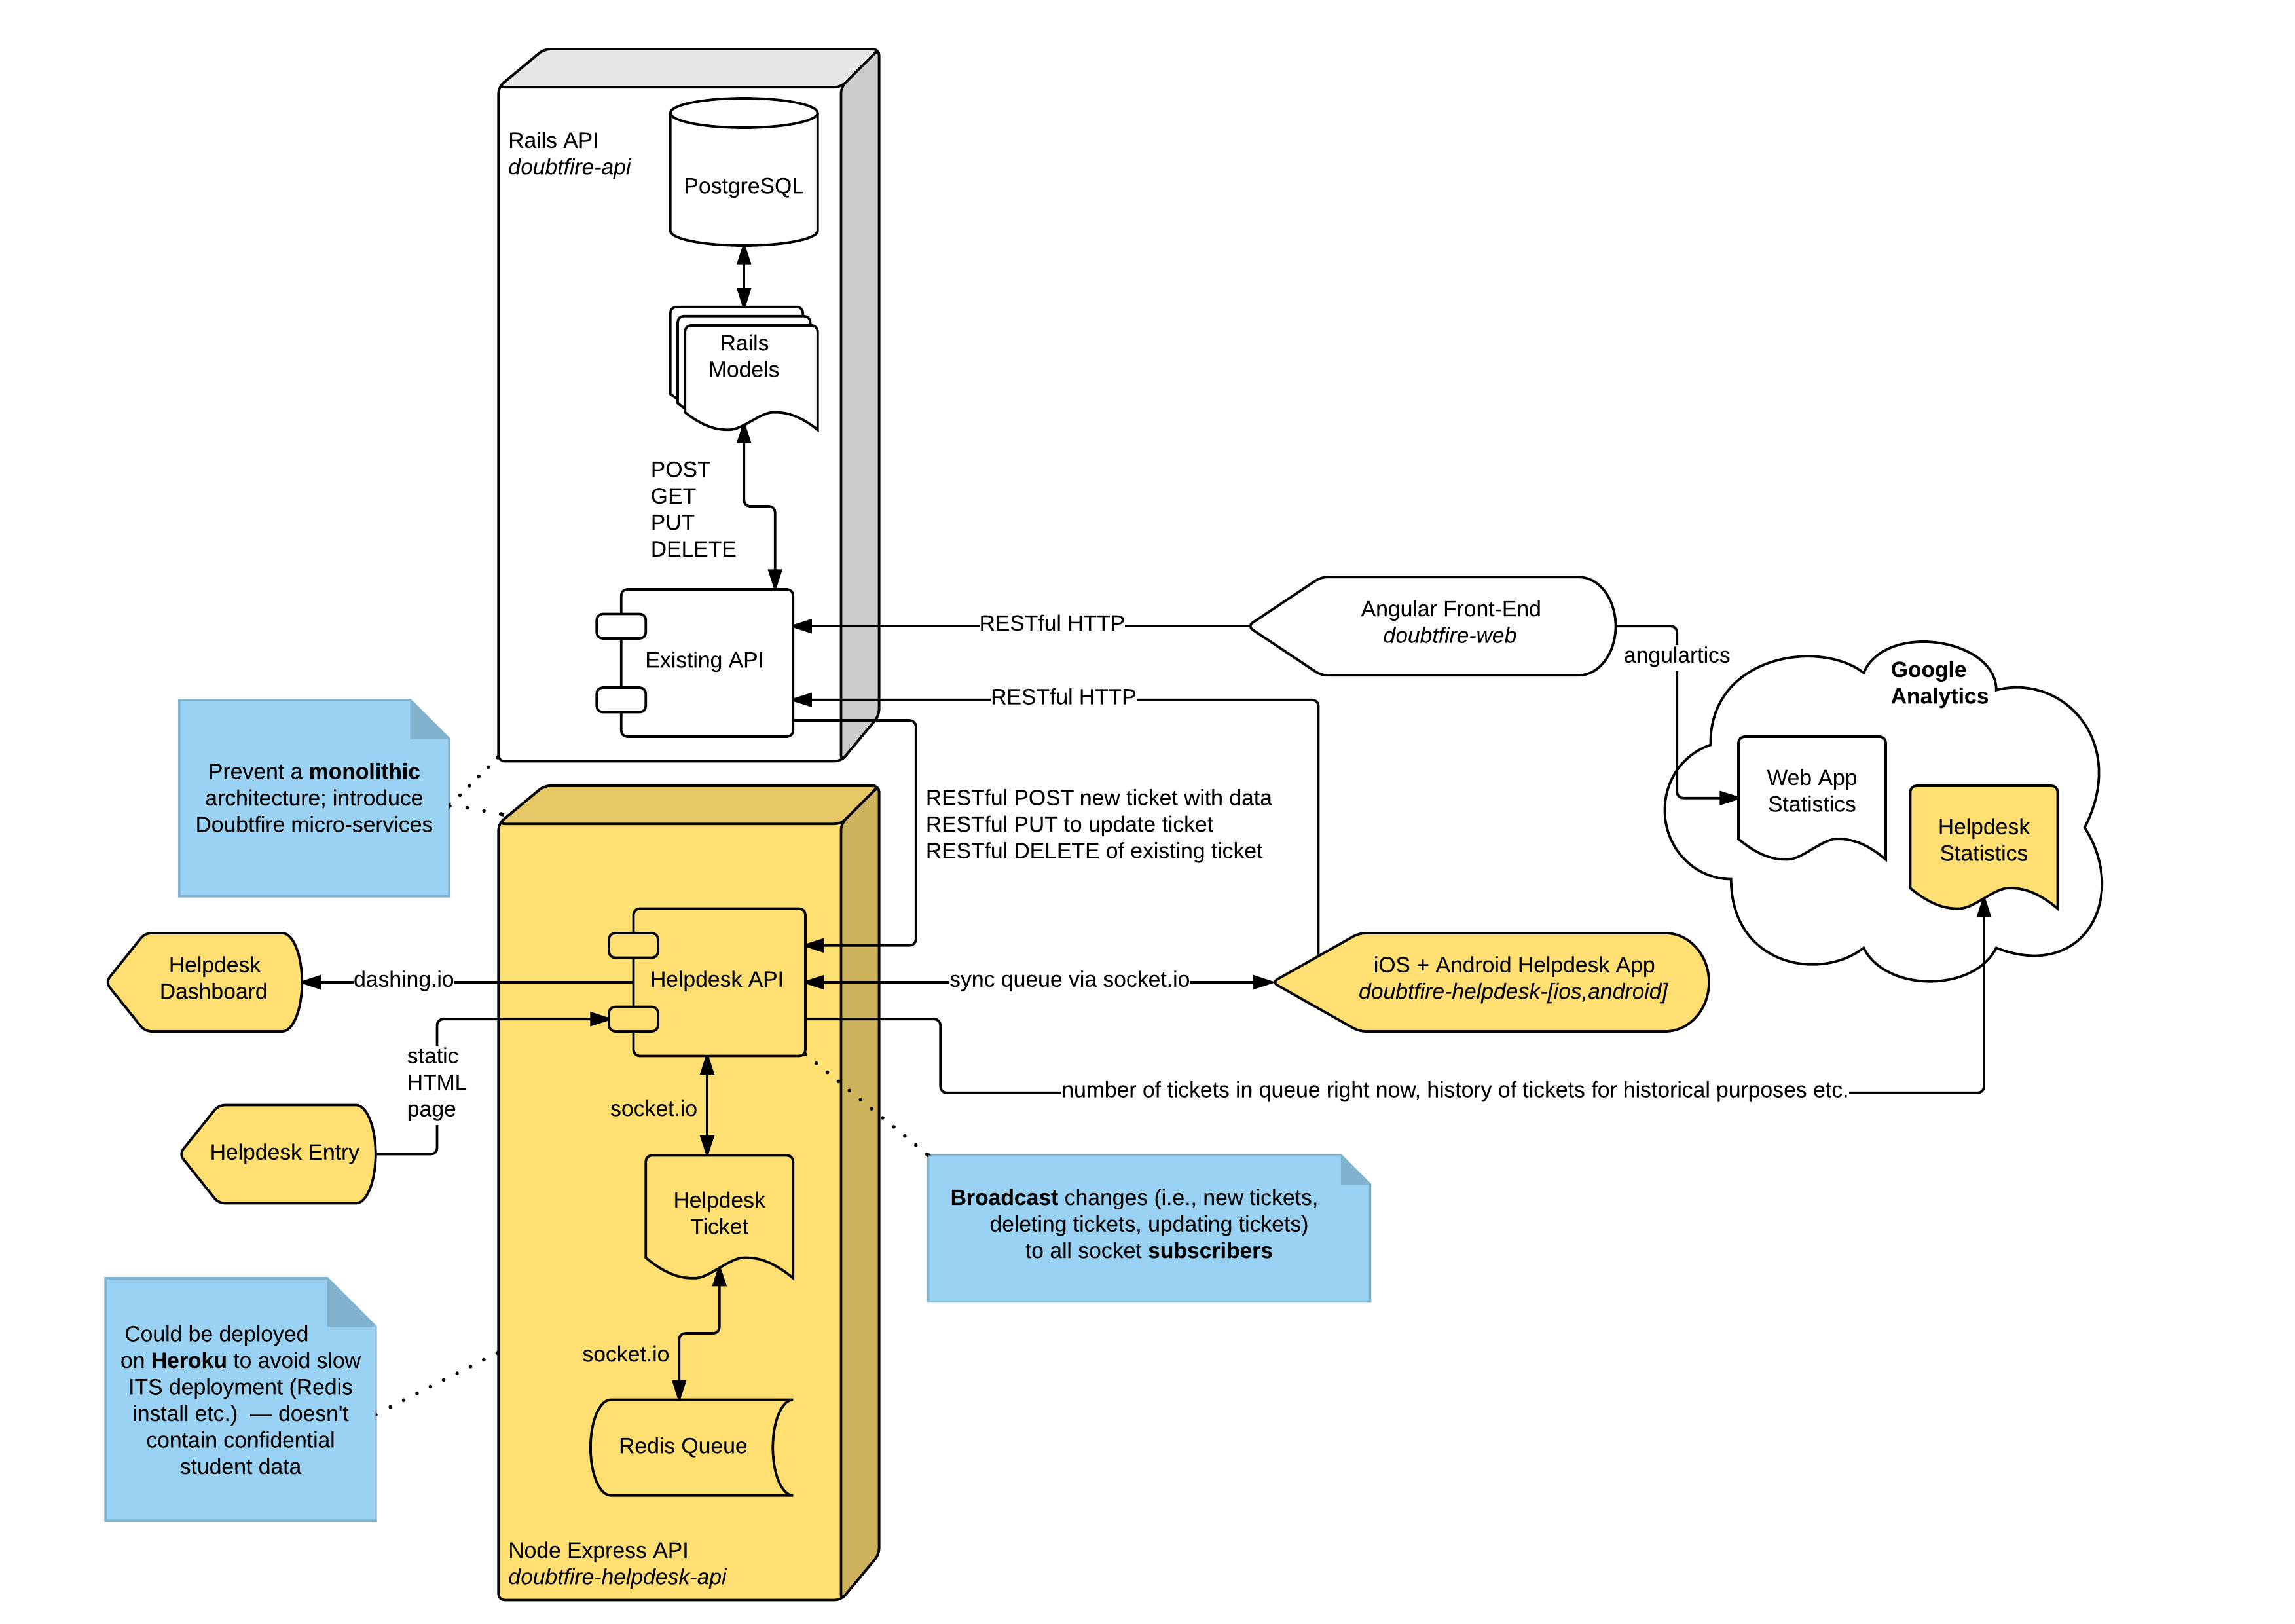
\includegraphics[angle=90, width=\textwidth]{8a0213b6-9fb0-4153-bd40-de3e6deebbff.png}
  \caption{High Level Architecture Diagram}
  \label{hla}
\end{figure}

\newpage

\appendix

\section{Supporting Use Case Images}
\label{sec:Supporting Images}

\begin{figure}[h!]
  \centering
  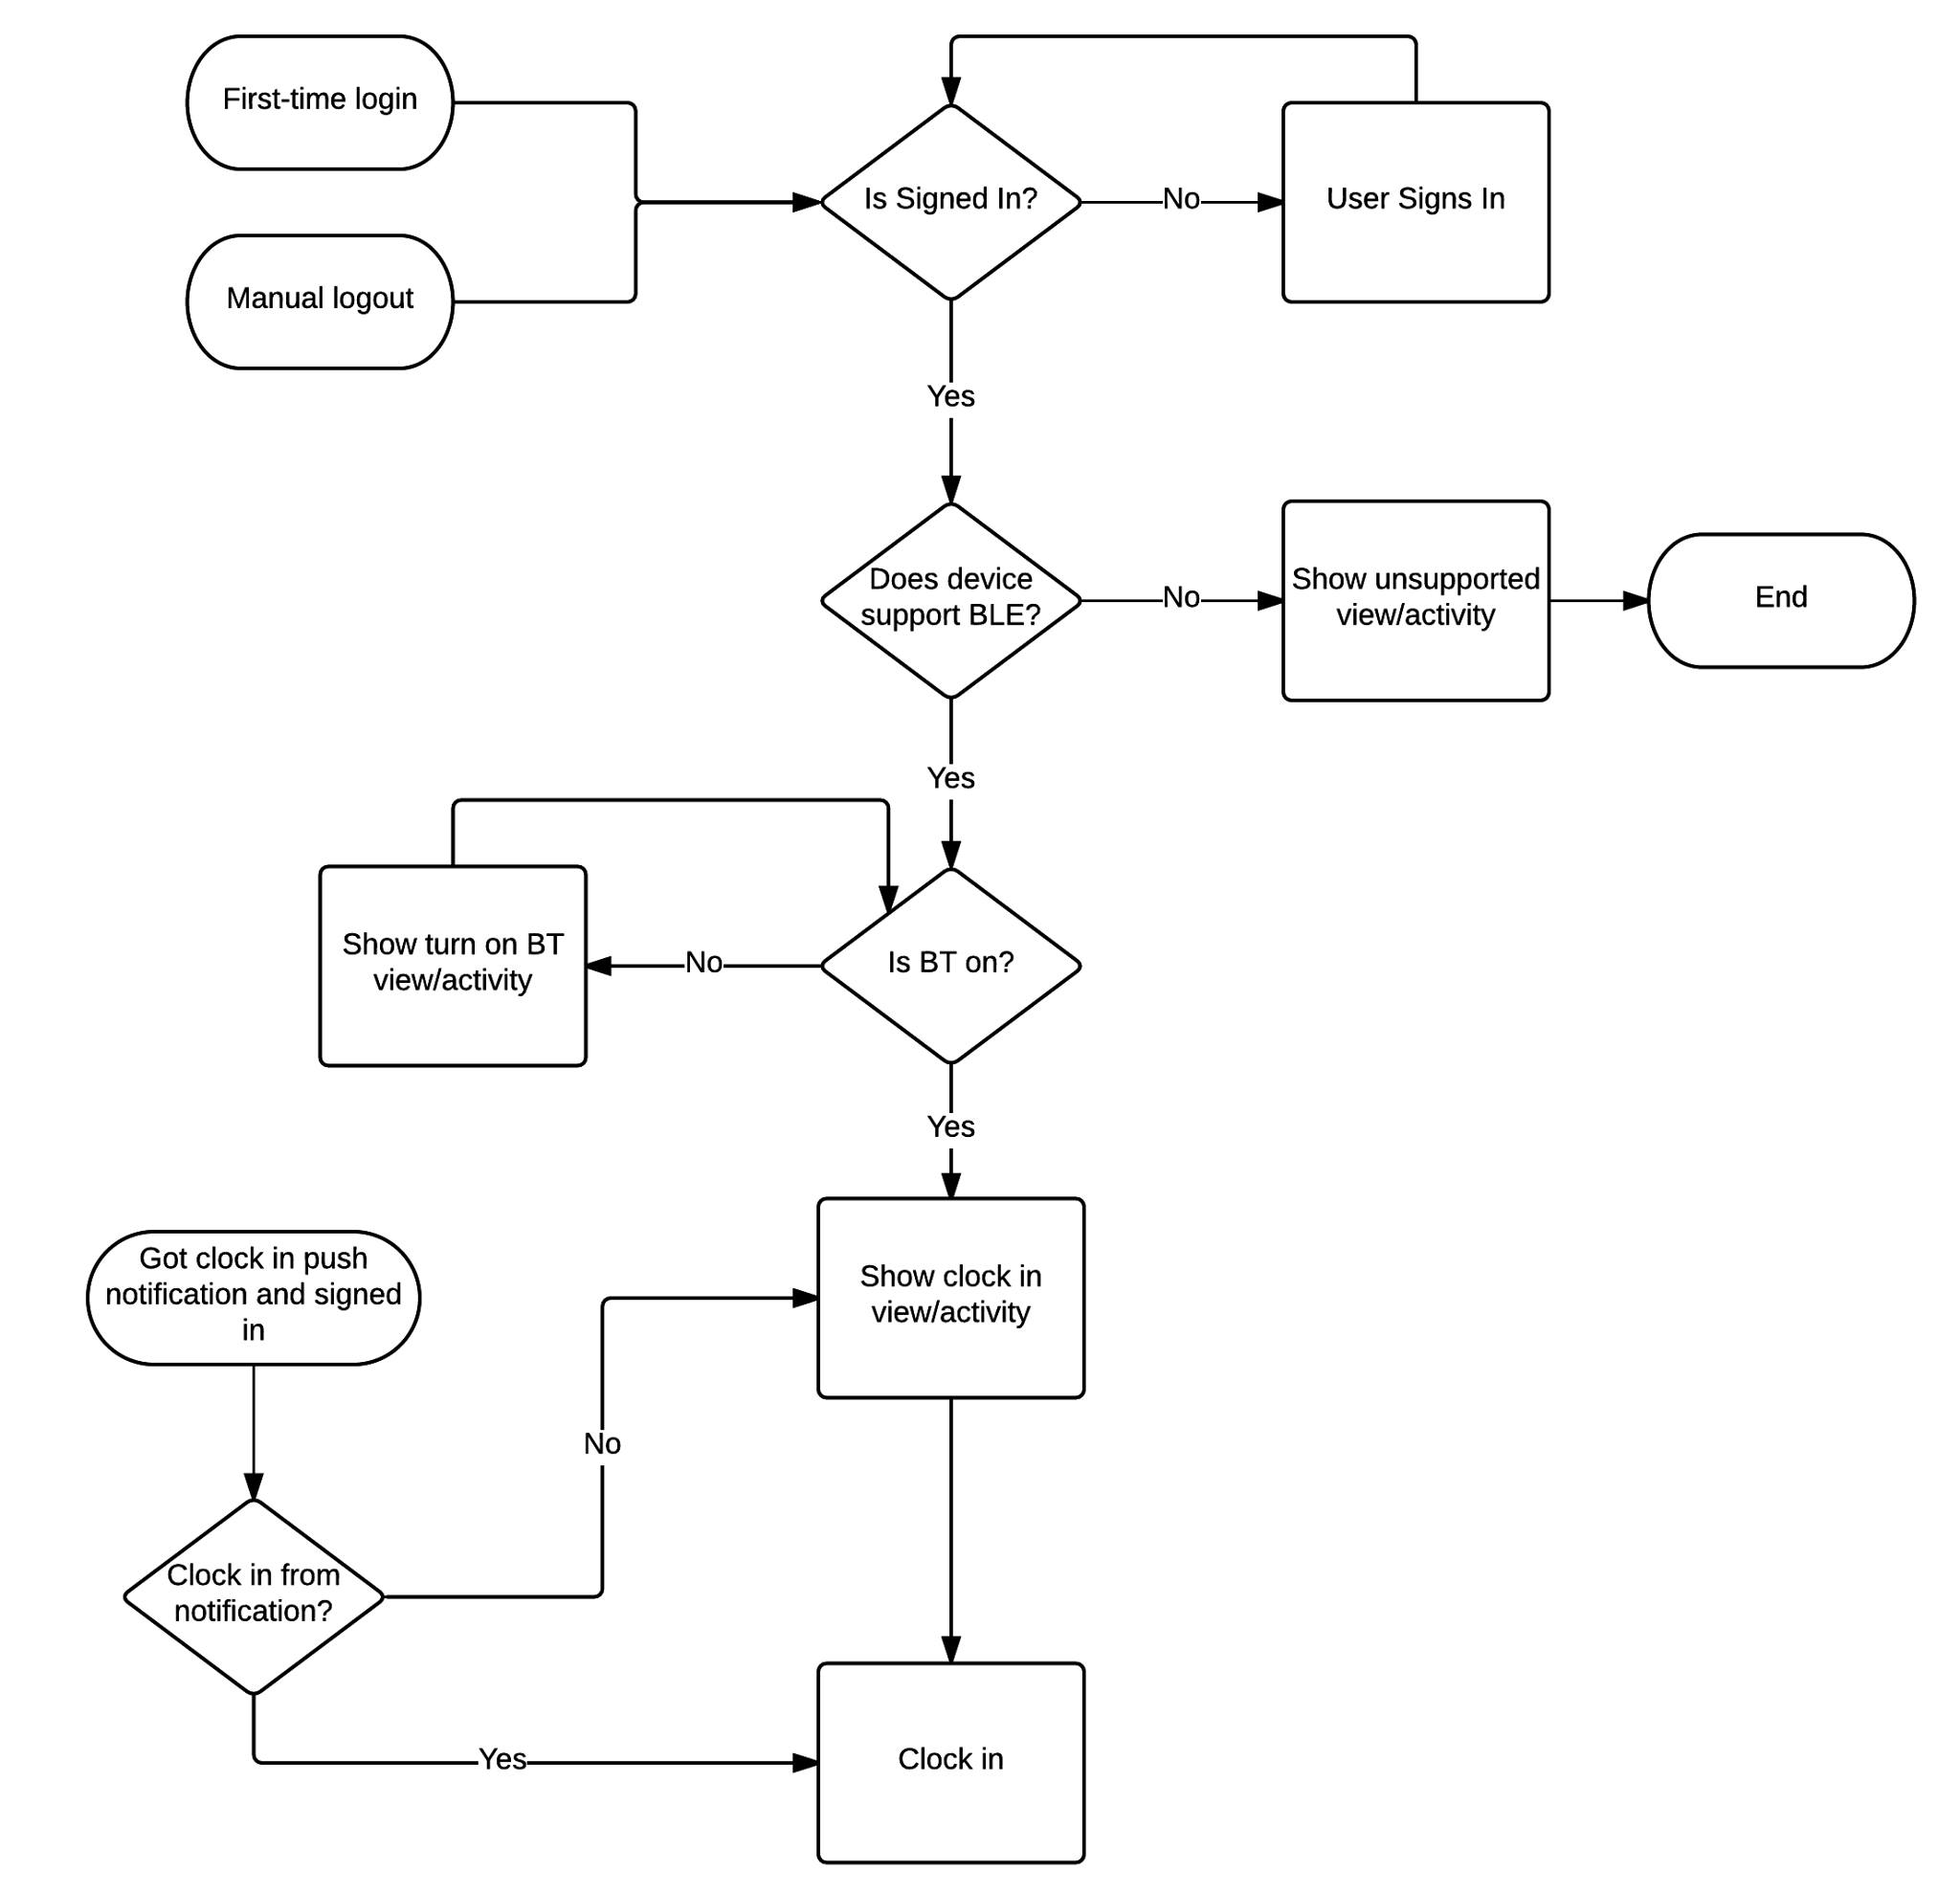
\includegraphics{b26d932a-a9db-4f4d-bb69-fb76f54ac074.jpeg}
  \caption{Workflow diagram for clocking on}
  \label{wd}
\end{figure}

\begin{figure}[p]
  \centering
  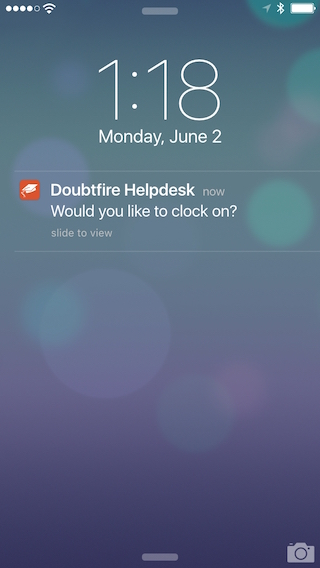
\includegraphics[]{4a9727edb2.jpg}
  \caption{Push notification to clock on}
  \label{pushnotif}
\end{figure}

\begin{figure}[p]
\centering
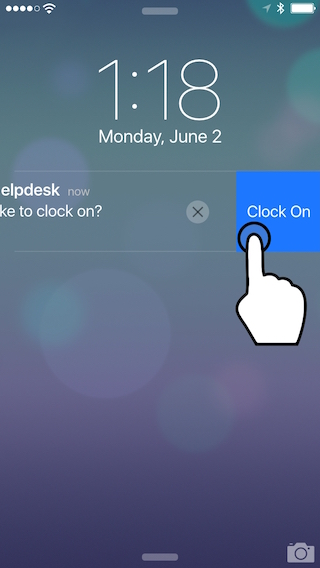
\includegraphics[]{cb0c91061e.jpg}
\caption{Clock on accept via notification}
\label{clockonnotif}
\end{figure}

\begin{figure}[p]
\centering
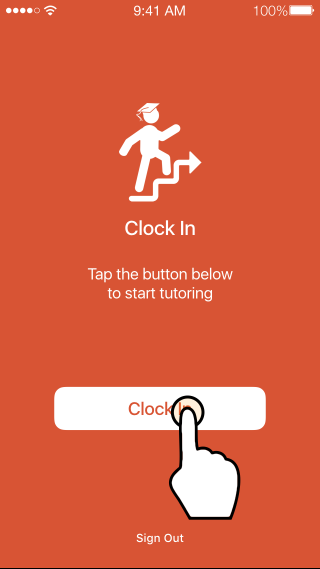
\includegraphics[]{3c23c7e0b0.png}
\caption{Clock on manually}
\label{clockonmanual}
\end{figure}

\end{document}
